\documentclass[tikz, border=5pt]{standalone}
\usetikzlibrary{arrows.meta}

\usepackage{bm}

\begin{document}

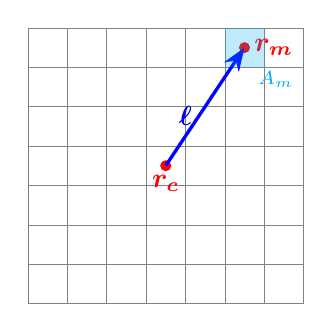
\begin{tikzpicture}[>=Stealth]
	\coordinate (C) at (1.75, 1.75);
	\coordinate (M) at (2.75, 3.25);

	\draw[step=0.5cm, gray, very thin] (0, 0) grid (3.5, 3.5);

	\fill[red] (C) circle [radius=2pt] node [below] {$\bm{r_c}$};
	\fill[red] (M) circle [radius=2pt] node [right] {$\bm{r_m}$};

	\draw[->, blue, very thick] (C) --  node [near start, above] {$\bm{\ell}$} (M);

	\fill[cyan, nearly transparent] (2.5, 3.0) rectangle (3, 3.5);

	\path[font=\scriptsize] (3.15, 2.85) node [cyan] {$A_m$};
\end{tikzpicture}

\end{document}
